\section{Data and Methodology}
\label{sec:data}

\subsection{Surveys:  KiDS, BOSS and 2dFLenS}
\label{sec:surveys}

The Kilo-Degree Survey \citep[KiDS,][]{dejong/etal:2013}, spans 1350 sq degrees split into two fields, one
equatorial and one southern.    Matched-depth imaging in nine bands spans the optical,
$urgi$, through to the near-infra-red, $ZYJHK_s$, where the
near-infra-red imaging was taken as part of the KiDS partner survey
VIKING \citep[the VISTA Kilo-degree INfrared Galaxy
survey,][]{edge/etal:2013}.  High quality seeing was
routinely allocated to the primary KiDS $r$-band VST-OmegaCAM observations, resulting in a
mean $r$-band seeing of 0.7 arcseconds, with a maximum of 0.8
arcseconds.  This combination of full-area spatial and wavelength
resolution over a thousand square degrees,
provides a unique weak lensing survey that allows for enhanced
control of systematic errors \citep{giblin/etal:inprep, hildebrandt/etal:inprep}.
This analysis uses data from the fourth KiDS
data release of 1006 square degrees of imaging, (hence the name KiDS-1000), which has an effective
area, after masking, of 777 square degrees.  KiDS is a public survey from the European Southern
Observatory, with data products freely accessible through the ESO
archive\footnote{KiDS data access: \href{http://kids.strw.leidenuniv.nl/DR4}{kids.strw.leidenuniv.nl/DR4}}.   

\citet{giblin/etal:inprep} presents a series of null-tests to validate the KiDS-1000 shear catalogue in five tomographic bins spanning a 
photometric redshift range of $0.1 < z_{\rm B} < 1.2$ \citep[see table 1 of][for the properties of each bin]{giblin/etal:inprep}.    
Meeting their requirement that any systematic detected induces less than a $0.1\sigma$ change in the inferred 
cosmic shear constraints on the clustering cosmological parameter $S_8 = \sqrt{\sigma_8 \Omega_m/0.3}$, they conclude that the shear catalogues are `science-ready'.
\citet{hildebrandt/etal:inprep} presents a cross-correlation clustering analysis to validate the fiducial KiDS-1000 photometric redshift calibration determined using the self-organising map (SOM) methodology of \citet{wright/etal:2020}.   The SOM identifies and excludes any galaxies that are poorly represented in the spectroscopic sample, in terms of their 9-band colours and magnitudes. The resulting `gold' photometric sample, with an accurately calibrated redshift distribution, is then re-simulated in the KiDS image simulations of \citet{kannawadi/etal:2019} in order to determine the shear calibration corrections for each tomographic bin, and an associated uncertainty \citep[see][for full details]{giblin/etal:inprep,hildebrandt/etal:inprep}.
 

The Baryon Oscillation Spectroscopic Survey
\citep[BOSS,][]{alam/etal:2015}, spans an effective area of 9329 square
degrees, with spectroscopic redshifts for 1.2 million luminous red
galaxies (LRG) in the redshift range $0.2<z<0.9$.   A range of
different statistical analyses of the clustering of BOSS galaxies have been used in combination with CMB
measurements, to set tight contraints on extensions to the standard
flat $\Lambda$CDM model \citep[see][and references
therein]{alam/etal:2017}.   We adopt the anisotropic clustering
measurements of \citet{sanchez/etal:2017} in this multi-probe analysis.
BOSS only overlaps with the equatorial stripe
of the KiDS survey, with 409 square degrees of the BOSS survey lying within
the KiDS-1000 footprint.  BOSS galaxies in this overlapping region are used as lenses in
our galaxy-galaxy lensing analysis, with an effective lens number density of 0.031
galaxies per square arcmin.  BOSS is a public survey from the third Sloan
Digital Sky Survey\footnote{BOSS data access: \href{https://data.sdss.org/sas/dr12/boss/lss/}{data.sdss.org/sas/dr12/boss/lss/}}.   

The two-degree Field Lensing Survey
\citep[2dFLenS,][]{blake/etal:2016}, spans 731 square degrees, with
spectroscopic redshifts for 70,000 galaxies out to $z<0.9$.   This
galaxy redshift survey from the Anglo-Australian Telescope was designed
to target areas already mapped by weak lensing surveys to facilitate `same-sky'
lensing-clustering analyses
\citep{johnson/etal:2017,amon/etal:2018,joudaki/etal:2018, blake/etal:2020}.
We use data from the 2dFLenS LRG sample that was targeted to match
the BOSS-LRG selection, but with sparser sampling.  2dFLenS
thus provides an additional sample of BOSS-like galaxies in the KiDS
southern stripe where there is 425 square degrees of overlap within
the KiDS-1000 footprint.  2dFLenS galaxies in this overlapping region are used as lenses in
our galaxy-galaxy lensing analysis, with an effective lens number density of 0.012
galaxies per square arcmin.  2dFLenS is a public survey\footnote{2dFLenS data
  access: \href{http://2dflens.swin.edu.au/data.html}{2dflens.swin.edu.au/data.html}}.   


\subsection{Cosmic Shear}
\label{sec:cosmic_shear}
The observed cosmic shear angular power spectrum, $C_{\epsilon \epsilon}(\ell)$, measures a combination of the distortions arising from weak gravitational lensing by large scale structures (labelled with a subscript `G') with a low-level contaminating astrophysical signal arising from the intrinsic alignment of galaxies with the large scale structures within which they are embedded (labelled with a subscript `I').   These contributions can be separated as
\be
\label{eq:cl_cosmicshear}
C^{(ij)}_{\epsilon \epsilon}(\ell) = C^{(ij)}_{\rm GG}(\ell) +
C^{(ij)}_{\rm GI}(\ell) + C^{(ij)}_{\rm IG}(\ell) + C^{(ij)}_{\rm II}(\ell)\;,
\ee
where the indices $i$ and $j$ indicate the five tomographic source samples.   The theoretical power spectrum are given by Limber-approximated projections with
\be
\label{eq:generallimber}
C^{(ij)}_{\rm ab}(\ell) = \int^{\chi_{\rm hor}}_0 \!\!\! \dd \chi\;
\frac{W^{(i)}_{\rm a} (\chi)\; W^{(j)}_{\rm b} (\chi)}{f^2_{\rm
    K}(\chi)}\; P_{\rm m, nl} \br{\frac{\ell+1/2}{f_{\rm K}(\chi)},z(\chi)}\;,
\ee
where ${\rm a,b} \in \bc{\rm I,G}$, $f_{\rm K}(\chi)$ is the comoving angular diameter distance and $\chi$ is the comoving radial distance which runs out to the horizon, $\chi_{\rm hor}$.  The weight functions, $W(\chi)$, encode information about the KiDS-1000 survey depth \citep[see equations 15 and 16 of][]{joachimi/etal:inprep}.   In the cases of power spectra that include intrinsic `I' terms, the weight function also encodes the intrinsic galaxy alignment model which we take to be the `NLA' model from \citet{bridle/king:2007}.   The cosmological information for this statistic is contained in both the geometric weight functions, $W(\chi)$, and in the evolution and shape of the non-linear matter power spectrum, $P_{\rm m, nl}(k,z)$, which we model using the halo formalism of \citet{mead/etal:2015}.   Weak lensing is therefore fairly unique as a cosmological probe, as it is sensitive to changes in both the distance-redshift relation and in the growth of structures.

We estimate the cosmic shear angular power spectrum through a linear transformation of the real-space two-point shear correlation function \citep{schneider/etal:2002}.  This approach circumvents the challenge of accurately determining the survey mask for a direct power spectrum estimate.  \citet{joachimi/etal:inprep} detail the apodisation advances that we have adopted for the transformation, in addition to the modelling that we use to account for the minor differences between the theoretical expectation of the true angular power spectrum in equation~\ref{eq:cl_cosmicshear} and the measured `band powers'.    
 
Figure~\ref{fig:Pkk} presents the \citet{asgari/etal:inprep} KiDS-1000 cosmic shear power spectra for the auto and cross-correlated tomographic bins.   Here we have constructed both E-mode (upper left) and B-mode (lower right) band powers in order to isolate any non-lensing B-mode distortions.     As expected from the analysis of \citet{giblin/etal:inprep}, the measured B-modes are found to be consistent with zero.   The measured E-modes can be compared to the theoretical expectation given the best-fit set of cosmological parameters from our joint multi-probe analysis in Section~\ref{sec:results}.



\begin{figure*}
        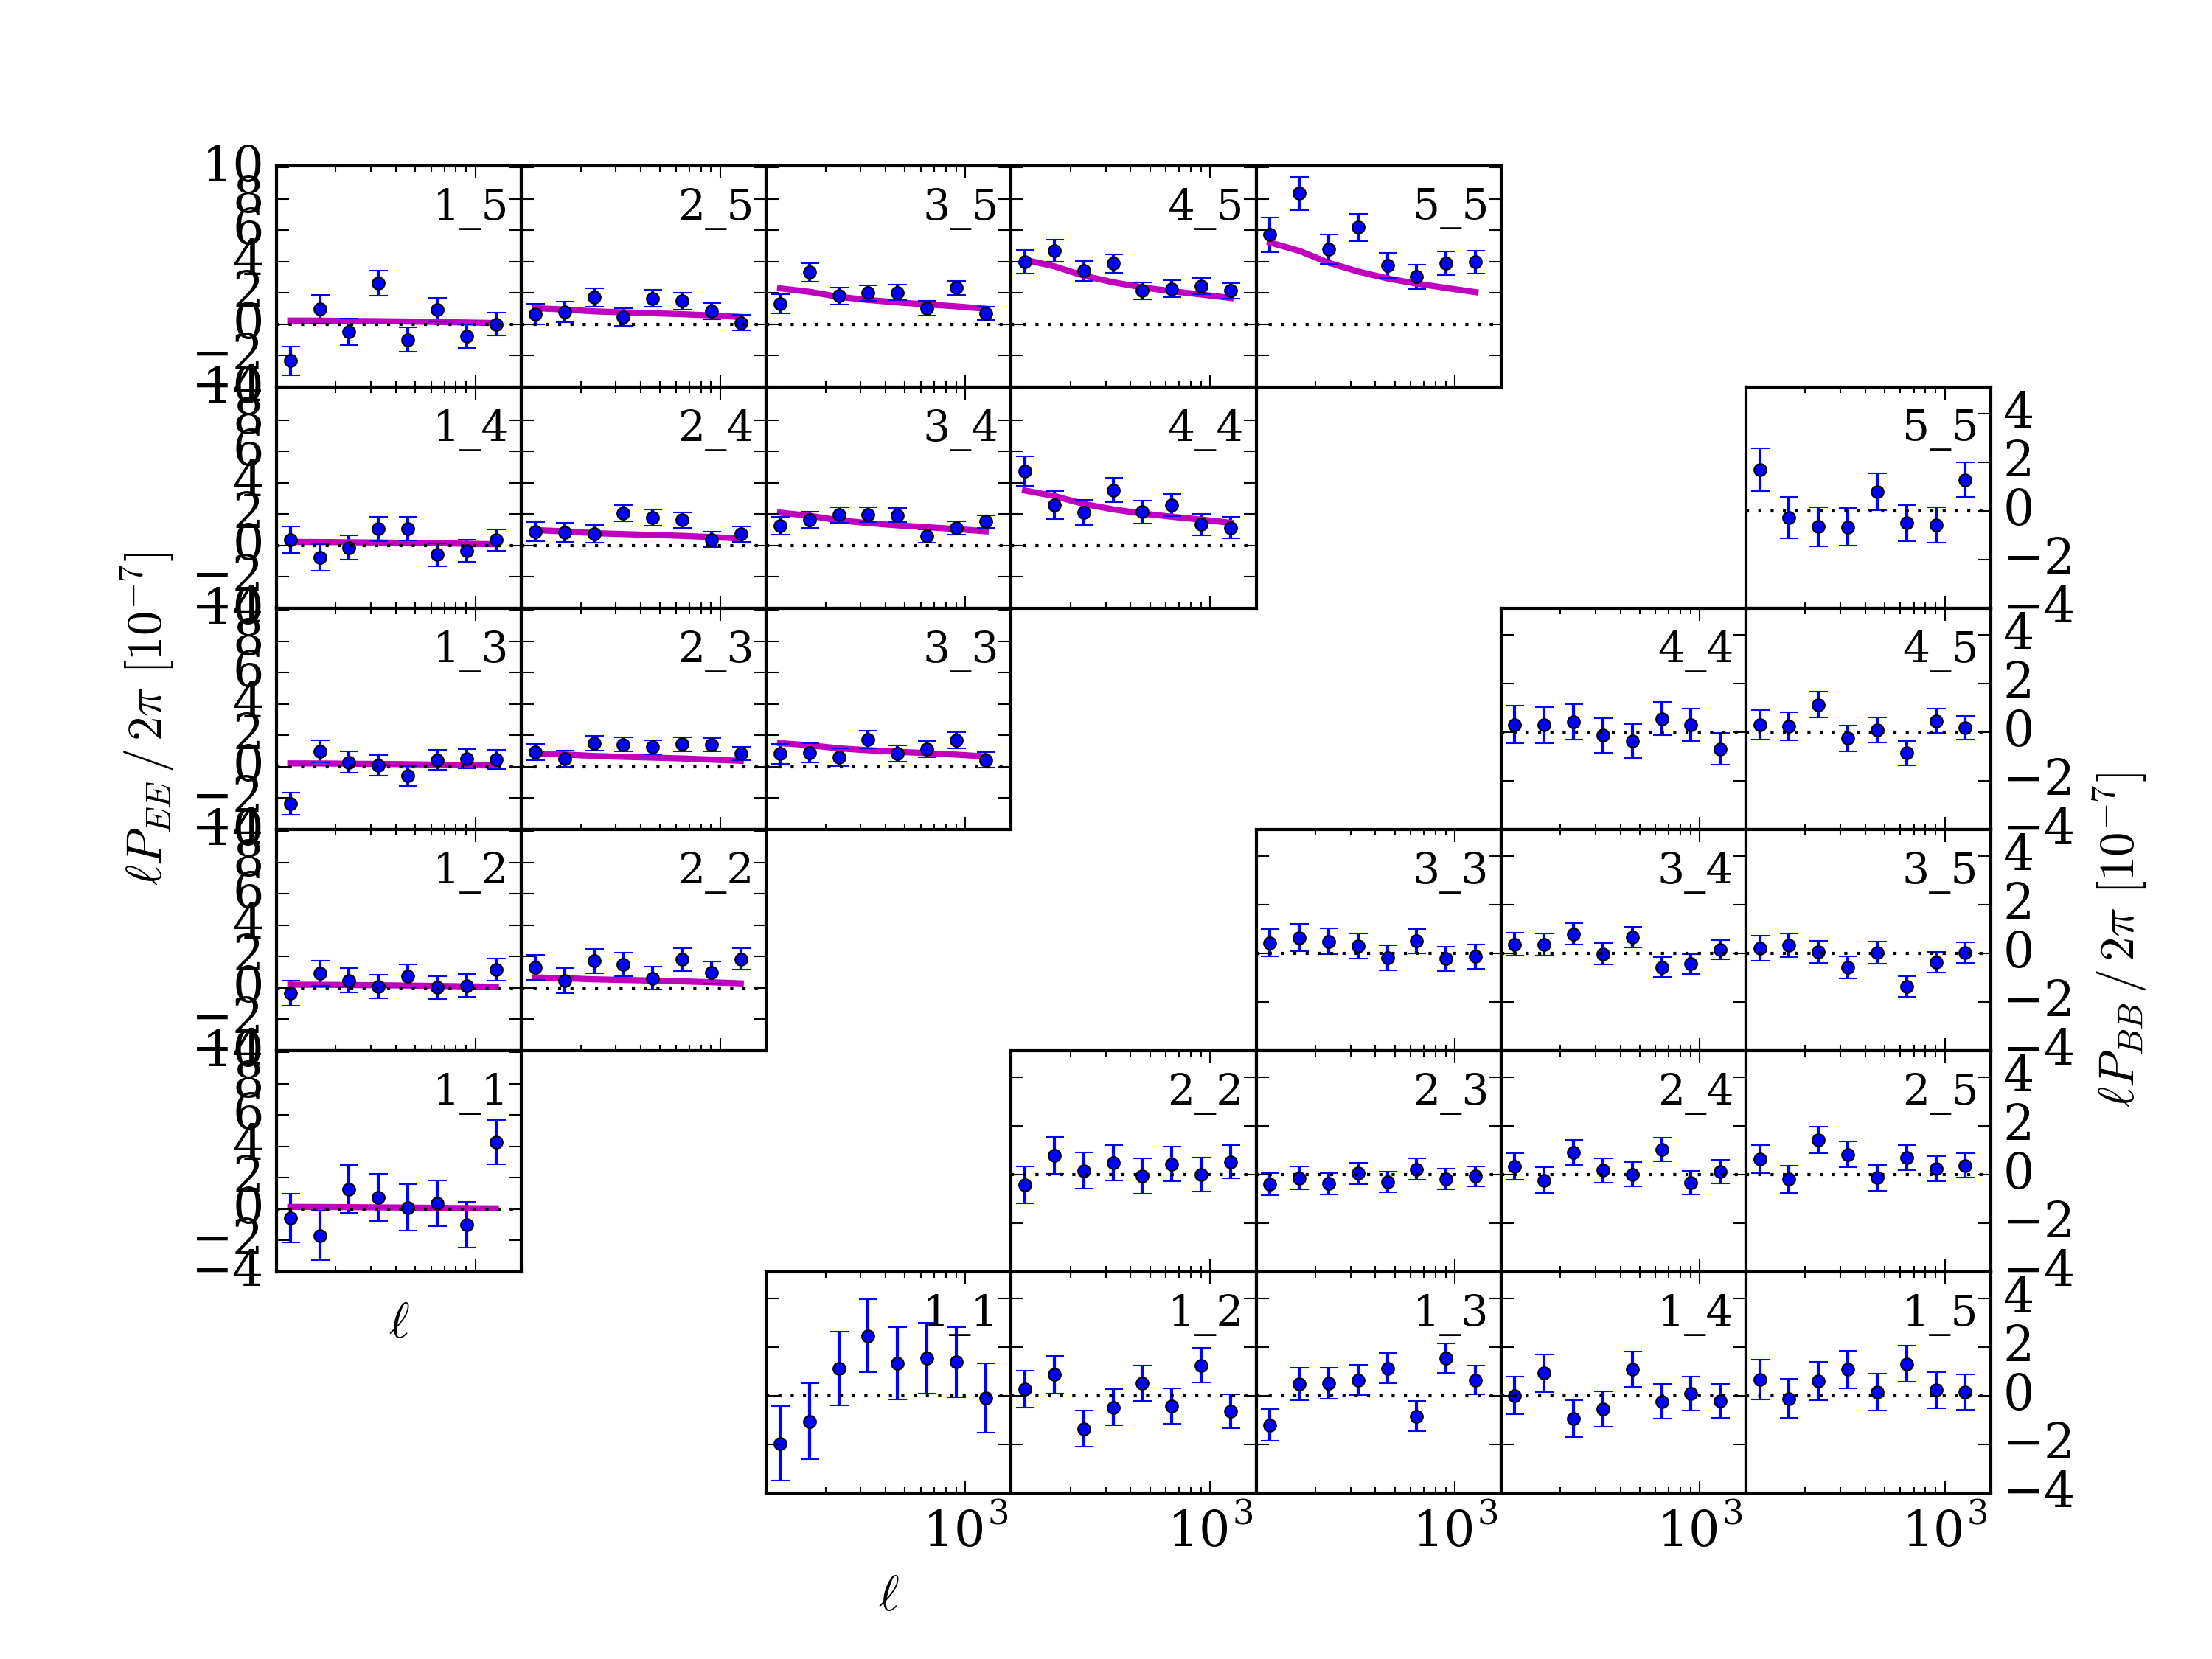
\includegraphics[width=\textwidth]{Data_Plots/Pkk/Pkk_K1000_2Dbins_v2_goldclasses_Flag_SOM_Fid_A.png}
        \caption{KiDS-1000 cosmic shear power spectra:  Tomographic
          band powers comparing the E-modes (upper left block) with the best-fit
          cosmological model from our combined multi-probe analysis
          \ch{TO DO}.  The tomographic
        bin combination is indicated in the upper right corner of each
      sub-panel.  The null-test B-modes (lower right block), are
      consistent with zero for both the full data vector, and each
     bin combination individually.}
        \label{fig:Pkk}
\end{figure*}

\subsection{Galaxy-Galaxy Lensing}
\label{sec:GGL}
Summary of Blake et al?


In Figure~\ref{fig:Pgk} we present the KiDS-1000 galaxy-galaxy lensing
power spectra, around lenses from the BOSS and 2dFLenS surveys.

\begin{figure*}
        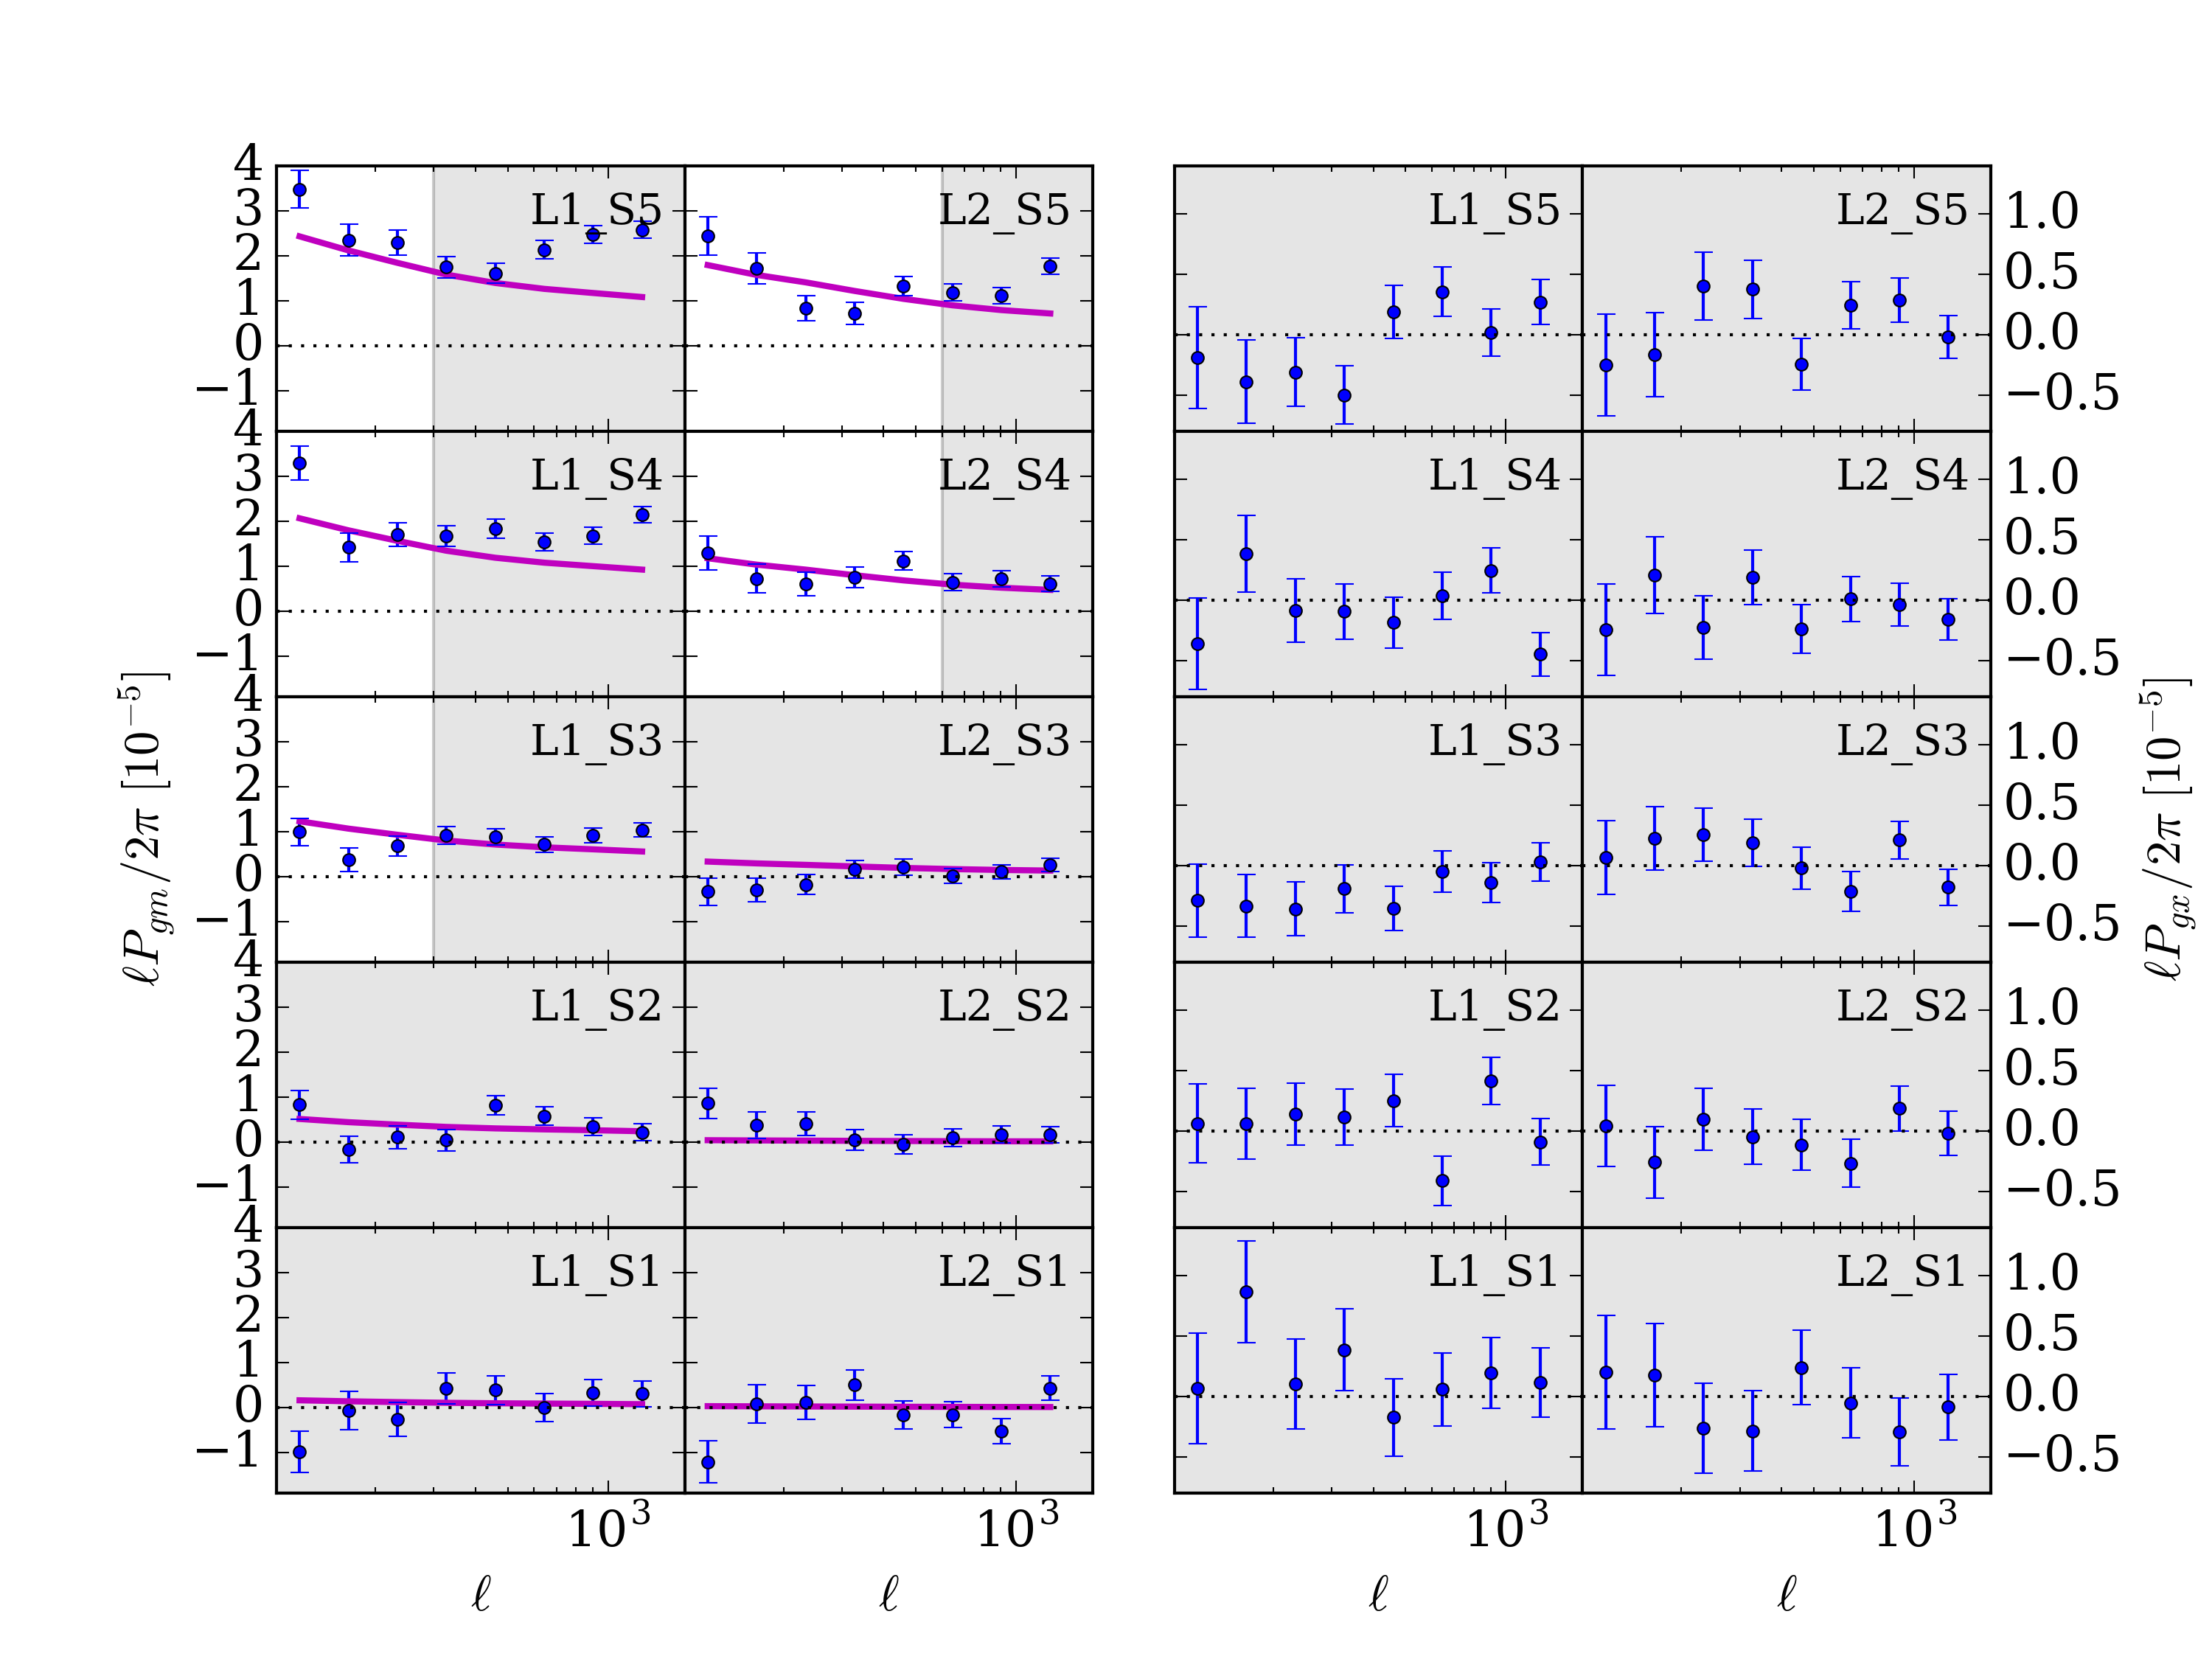
\includegraphics[width=\textwidth]{Data_Plots/Pgk/Pgk_K1000_2Dbins_v2_goldclasses_Flag_SOM_Fid_A.png}
        \caption{KiDS-1000 galaxy-galaxy lensing power spectra:
          Tomographic band powers comparing the E-modes (left block)
          with the best-fit
          cosmological model from our combined multi-probe analysis
          \ch{TO DO}.  The tomographic 
        bin combination of BOSS and 2dFLenS lenses (L) with KiDS-1000
        sources (S), is indicated in the upper right corner of each
        sub-panel.  Data within grey-regions are not included in the cosmological analysis.
        The null-test B-modes (right block), are
      consistent with zero for both the full data vector, and each
     bin combination individually \ch{TO DO}.}
        \label{fig:Pgk}
\end{figure*}

\subsection{Anisotropic Galaxy Clustering}
\label{sec:clustering}
Summary of \citet{sanchez/etal:2017}

In Figure~\ref{fig:wedges} we present the BOSS-DR12 anisotropic
clustering wedges.
\begin{figure*}
        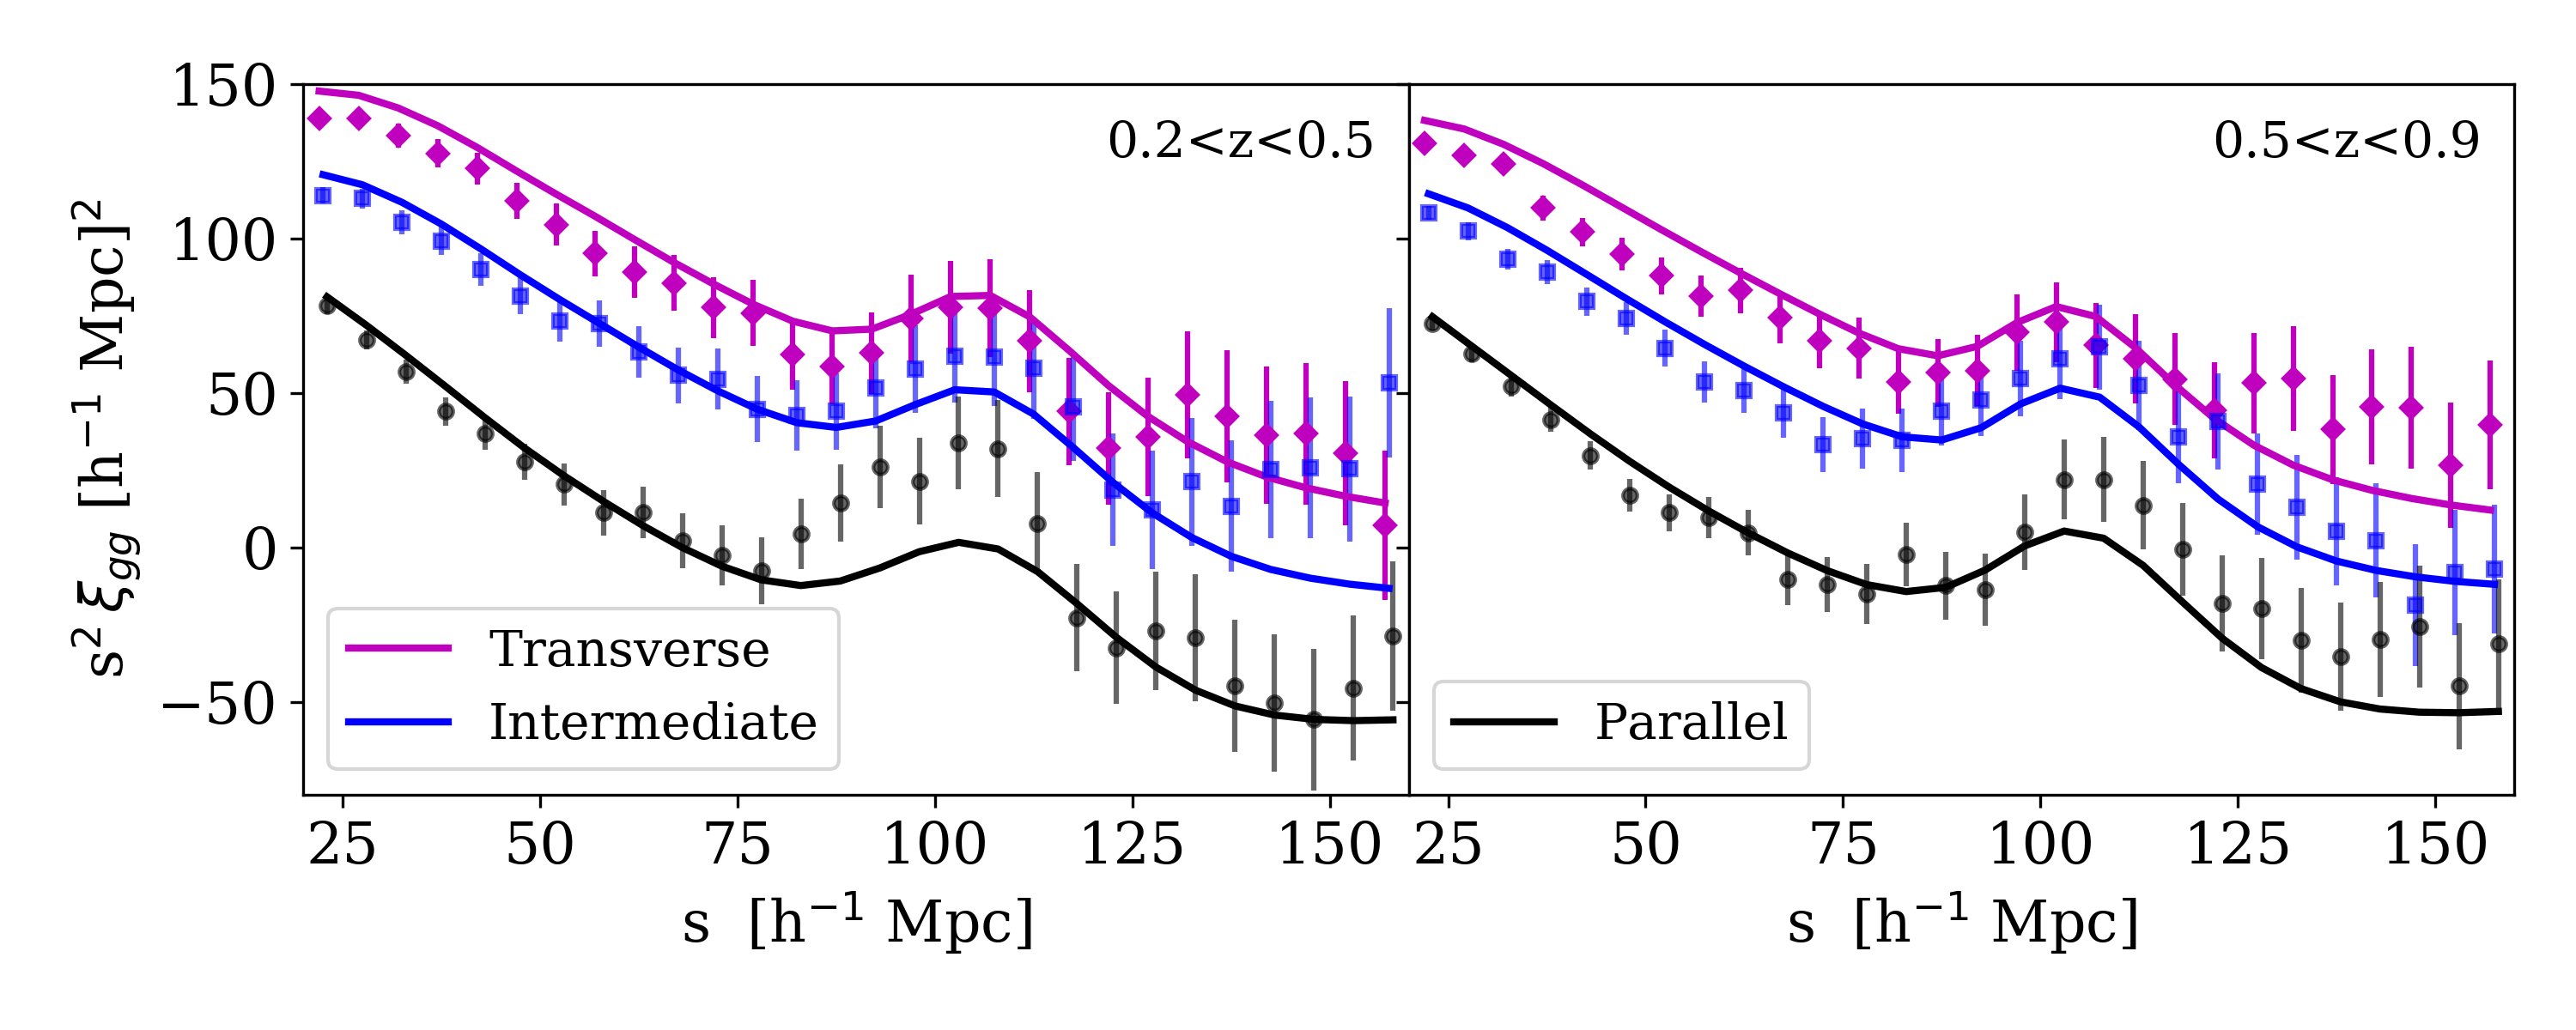
\includegraphics[width=\textwidth]{Data_Plots/clustering_wedges/BOSS_Sanchez_wedges.png}
        \caption{BOSS-DR12 anisotropic clustering from \citet{sanchez/etal:2017}:
          The transverse (pink), intermediate (blue) and parrallel
          (black) clustering wedges in two redshift bins, compared 
          with the best-fit
          cosmological model from our combined multi-probe analysis
          \ch{TO DO}.}
        \label{fig:wedges}
\end{figure*}

\subsection{Covariance}
\label{sec:Cov}
Summary of \citet{joachimi/etal:inprep}

